%!TEX program = lualatex

\documentclass{tufte-handout}
\usepackage{hyperref}
\usepackage{amsmath}
\usepackage{titlesec}
\usepackage{framed}
%\usepackage{todonotes}
\usepackage{arydshln}
\usepackage{fontawesome}
%\usepackage{fontspec}
\usepackage{pdfpages}
\usepackage{csquotes}
\MakeOuterQuote{"}
%\setmainfont{Palatino Linotype}

\titleformat
{\part} % command
[display] % shape
{\bfseries\Large\itshape} % format
{Story No. \ \thechapter} % label
{0.5ex} % sep
{
    \rule{\textwidth}{1pt}
    \vspace{1ex}
    \centering
} % before-code
[
\vspace{-0.5ex}%
\rule{\textwidth}{0.3pt}
] % after-code

% Set up the images/graphics package
\usepackage{graphicx}
\setkeys{Gin}{width=\linewidth,totalheight=\textheight,keepaspectratio}
\graphicspath{{syllabus-img/}}

\title{Social and Emotional Approaches to Learning and Teaching}
\author{Dr. Jeremy Price}
\date{Fall 2015}  % if the \date{} command is left out, the current date will be used

% The following package makes prettier tables.  We're all about the bling!
\usepackage{booktabs}

% The units package provides nice, non-stacked fractions and better spacing
% for units.
\usepackage{units}

% The fancyvrb package lets us customize the formatting of verbatim
% environments.  We use a slightly smaller font.
\usepackage{fancyvrb}
\fvset{fontsize=\normalsize}

% Small sections of multiple columns
\usepackage{multicol}

% Provides paragraphs of dummy text
\usepackage{lipsum}

\usepackage{microtype}

\usepackage{newpxtext,newpxmath}
\useosf % old-style figures in text, not in math

% These commands are used to pretty-print LaTeX commands
%\newcommand{\doccmd}[1]{\texttt{\textbackslash#1}}% command name -- adds backslash automatically
%\newcommand{\docopt}[1]{\ensuremath{\langle}\textrm{\textit{#1}}\ensuremath{\rangle}}% optional command argument
%\newcommand{\docarg}[1]{\textrm{\textit{#1}}}% (required) command argument
%\newenvironment{docspec}{\begin{quote}\noindent}{\end{quote}}% command specification environment
%\newcommand{\docenv}[1]{\textsf{#1}}% environment name
%\newcommand{\docpkg}[1]{\texttt{#1}}% package name
%\newcommand{\doccls}[1]{\texttt{#1}}% document class name
%\newcommand{\docclsopt}[1]{\texttt{#1}}% document class option name

\newcommand{\gentopic}[1]{\begin{fullwidth}\begin{center}\faKey \textsf{#1}\end{center}\end{fullwidth}}
\newcommand{\tabpq}{\faQuestionSign\medspace\textit{Priming Questions}}
\newcommand{\tabread}{\faBook\medspace\textit{Readings}}
\newcommand{\tabperformance}{\faTasks\medspace\textit{Performances}}
\newcommand{\tabdt}{\faCalendar\medspace\textit{Week Of}}
\newcommand{\tabcheckin}{\faPagelines\medspace\textit{Check-In Performances}}
\newcommand{\tabbreak}{\begin{fullwidth}\begin{center}\faAsterisk\faAsterisk\faAsterisk\\\end{center}\end{fullwidth}}
\newcommand{\specialweek}[1]{\begin{fullwidth}\begin{center}\textbf{\faBullhorn\medspace Special Week: #1 \medspace\faBullhorn}\end{center}\end{fullwidth}}
\newenvironment{tabsched}
	{\small
	\begin{tabular}{p{1.5in}p{4.5in}}
	\midrule}
	{\midrule
	\end{tabular}
	\normalsize}

\newenvironment{specweek}
	{\begin{center}
		\fontseries{b} \faBullhorn \medspace Special Week: }
		{\medspace \faBullhorn \fontseries{m}
	\end{center}}

\newcommand{\weekone}{August 17-21}
\newcommand{\weektwo}{August 24-28}
\newcommand{\weekthree}{August 31-September 4}
\newcommand{\weekfour}{September 7-11}
\newcommand{\weekfive}{September 14-18}
\newcommand{\weeksix}{September 21-25}
\newcommand{\weekseven}{September 28-October 2}
\newcommand{\weekeight}{October 5-9}
\newcommand{\laborday}{Labor Day on Monday, September 7 (no class)}
\newcommand{\roshhashanah}{Rosh Hashanah on Monday, September 14 (class via VoiceThread)}
\newcommand{\yomkippur}{Yom Kippur on Wednesday, September 23 (class via VoiceThread)}
\newcommand{\finisemester}{\begin{fullwidth}\begin{center}\large\textbf{\faFlagCheckered Last Day of Class, Wednesday, October 7 \faFlagCheckered}\normalsize\end{center}\end{fullwidth}}

% Set up the spacing using fontspec features
\renewcommand\allcapsspacing[1]{{\addfontfeature{LetterSpace=15}#1}}
\renewcommand\smallcapsspacing[1]{{\addfontfeature{LetterSpace=10}#1}}

\begin{document}

\maketitle% this prints the handout title, author, and date

\begin{abstract}
Welcome to EDUC1099, Social and Emotional Approaches to Learning and Teaching. Blah blah blah blah.\end{abstract}

\bigskip

%\begin{fullwidth}
	\begin{center}
		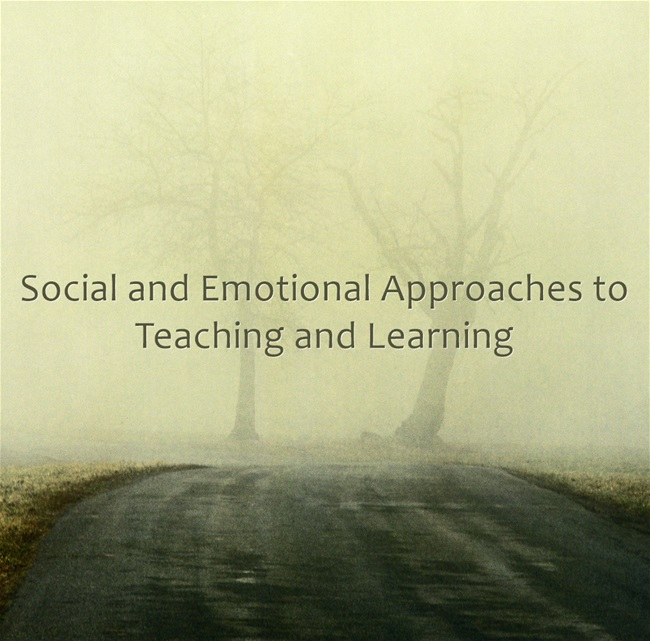
\includegraphics[width=0.40\linewidth]{sealt-logo.jpg}

		\bigskip

		\Large
		\enquote{It seems to me that that, finally, is what good teaching is all about\ldots Somehow or another, skill and knowledge are integrated into some kind of a human connection.}\\- Mike Rose
		\normalsize
	\end{center}
%\end{fullwidth}

\input{syllabus-files/professor-info}

\newpage

\part{The EDUC1099 Contract}

\begin{fullwidth}

\input{syllabus-files/undergraduate-course_contract}

\end{fullwidth}

\newpage

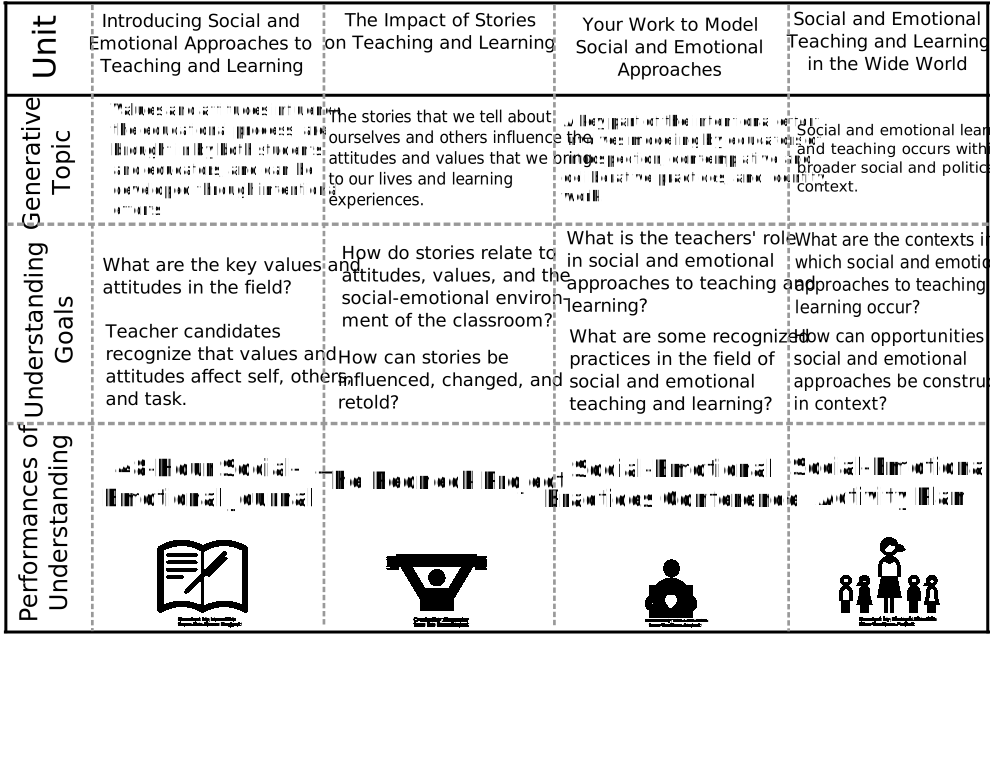
\includepdf[angle=90,width=5in,pages=1,pagecommand=\part{Course Map}]{sealt}

\newpage

\part{Course Practices and Routines}

\begin{marginfigure}%
	\begin{center}
		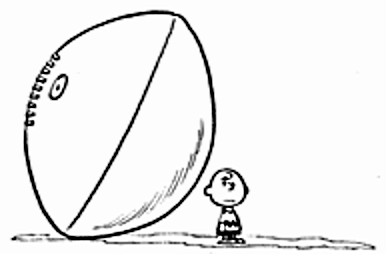
\includegraphics[width=1\linewidth]{cp-pic3.png}
	\end{center}
\end{marginfigure}

\input{syllabus-files/universal_learning}

\input{syllabus-files/attendance}

\input{syllabus-files/ooops_days}

\input{syllabus-files/email}

\input{syllabus-files/assignments}

\newpage

\part{Performances of Understanding}

\begin{marginfigure}%
	\begin{center}
		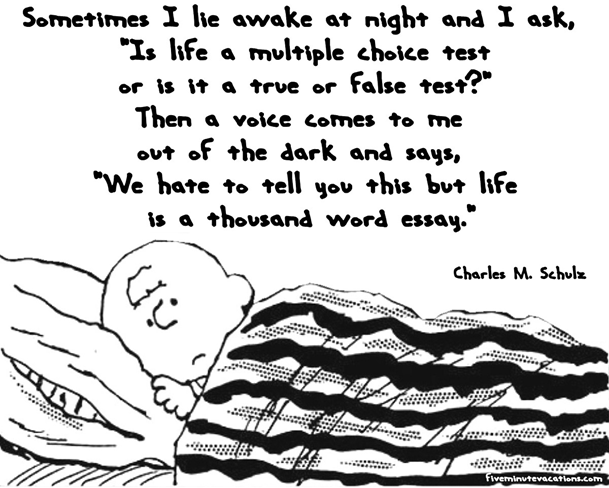
\includegraphics[width=1\linewidth]{lp-pic.png}
	\end{center}
\end{marginfigure}

\newthought{Performances of Understanding are a way for you to demonstrate what you understand while also building your understanding.} The \textit{Performances of Understanding}\footnote{Performances of Understanding are a concept from the Teaching for Understanding framework.} are what you produce in each of the 4 units of the course. Each of these Performances are designed to not only help me see what you understand, but also to help you deepen your knowledge and develop your skills around the use of technology in teaching and learning. You will receive a \textsf{Project Package} at the beginning of each unit which will include more specifics about what I expect from you, including a copy of the rubric that I will be using to evaluate your work. In addition to the Culminating Performances themselves, you will engage in Check-In Performances to help you get ready for the Culminating Performances.

\section{Unit 1:  Introducing Social and Emotional Approaches to Teaching and Learning}

In this unit, we will be exploring a framework for social and emotional approaches to teaching and learning. We will see how this framework intersects with the real lives of teachers and learners and the work in which they engage together. As a way to help you make these connections, you will be keeping a two-day journal in which you document when aspects of this framework intersect with your own experiences as a learner. You will then write a comprehensive, analytical, and rigorous reflection on what happened, how these experiences intersected with the framework, and how you now see things differently.

\medskip\noindent\textit{$\mapsto$ Your 48-Hour Social-Emotional Journal is worth \textbf{20 points}.}

\section{Unit 2: The Impact of Stories on Teaching and Learning}

When examining the social and emotional aspects of teaching and learning, it is important to recognize the stories we tell about ourselves, the stories we construct around others, and the stories that others tell about us. The story of the "redneck" is one that is intertwined with the cultural history of Appalachia, and is mostly not flattering. We will learn about the history of this phrase, learn about its significance, and work to "re-write" its meaning through creative artifacts. This re-writing is important to help students who may live out the stories written for them instead write the stories and live the lives they prefer.

\medskip\noindent\textit{$\mapsto$ Your Redneck Project is worth \textbf{20 points}.}

\section{Unit 3: Your Work to Model Social and Emotional Approaches to Teaching and Learning}

Modeling is one of the most powerful tools for teaching. It is therefore important to model social and emotional practices in your own teaching and learning lives as an educator. Each person in the class will select a social-emotional practice and conduct research into what it is, what purpose it serves, how it works, and what the potential outcomes are. You will create a short poster presentation for a Social-Emotional Practices Conference. You will be able to engage classmates in conversation about these practices.

\medskip\noindent\textit{$\mapsto$ Your presentation in the Social-Emotional Practices Conference is worth \textbf{20 points}.}

\subsection{Unit 4: Social and Emotional Teaching and Learning in the Wide World}

One of the most important jobs of an educator is to facilitate an environment to promote learning, and planning this environment is a necessary part of this process. As such, as your last performance, you will be planning an activity that incorporates principles and practices of social-emotional learning and teaching. This plan is a condensed version of the lesson plan format you will be expected to write later in your career as a teacher education candidate. I hope that you will continue

\medskip\noindent\textit{$\mapsto$ Your Social-Emotional Activity Plan is worth \textbf{20 points}.}

\section{Cross-Unit Considerations}

Blah

\medskip\noindent\textit{$\mapsto$ These combined considerations are worth \textbf{20 points}.}

\section{Course Point Breakdown}

\marginnote{90-100 points is an A, 80-89 points is a B, 70-79 points is a C, 65-69 is a D, 64 or less is an F.}Keep in mind that \emph{\textbf{you earn your grade}}. I do not "give" you a grade. As a teacher, I place a great deal of emphasis on becoming aware of learning processes and progress. \emph{This is a practice that is important to bring to your own students,} so I want to give you a head start.

\bigskip

\begin{tabular}{clr}
	\toprule
	Unit & Performance & Points \\
	\midrule\midrule
	1 & 48-Hour Social-Emotional Journal & 20 \\
	\midrule
	2 & The Redneck Project & 20 \\
	\midrule
	3 & Social-Emotional Practices Conference & 20 \\
	\midrule
	4 & Social-Emotional Activity Plan & 20 \\
	\midrule
	ALL & Check-In Performances, Participation, and Growth & 20 \\
	\midrule\midrule
	\multicolumn{2}{l}{\textbf{Total}} & \textbf{100} \\
	\bottomrule
\end{tabular}

\newpage

\part{\faCalendar\medspace Course Schedule \medspace\faCalendar}

\begin{marginfigure}
	\begin{center}
		
\includegraphics[width=0.4\linewidth]{sc-pic.png}
	\end{center}
\end{marginfigure}

\medskip

\section{Check-In and Culminating Performances of Understanding Due Dates}
\begin{tabular}{clr}
	\toprule
	Unit & Performance & Due Date \\
	\midrule\midrule
	1 & What Do I Notice? & August 21 \\
	& 48-Hour Social-Emotional Journal & August 31 \\
	\midrule
	2 & Re-Remembering Rednecks & September 4 \\
	& The Redneck Project & September 14 \\
	\midrule
	3 & Practices Organizer & September 18 \\
	& Social-Emotional Practices Conference & September 28 \\
	\midrule
	4 & Activity Organizer & October 2 \\
	& Social-Emotional Activity Plan & October 12 \\
	\bottomrule
\end{tabular}

%\begin{fullwidth}
	\section{Unit 1: Introducing Social and Emotional Approaches to Teaching and Learning}
%\end{fullwidth}

\gentopic{Values and attitudes influence the educational process, are brought in by both students and educators,\\and can be developed through intentional efforts.}


\begin{tabsched}
	\tabdt & \weekone \\
	\midrule
	\tabpq & What are some of the rules of the "program" for "doing school"? \\
	& Should an effort be made to "deprogram" students from "doing school"? \\
	& What does the author mean by "surprise," and why is surprise important for learning? \\
	\midrule
	\tabread & How Deprogramming Kids From How To Do School Could Improve Learning (\url{http://goo.gl/pnkkRM}) \\
	& Surprise Journal: Notice the Unexpected (\url{http://goo.gl/h2ESqJ}) \\
	\midrule
	\tabcheckin & \textbf{What have you noticed?} Due Friday, August 21 \\
\end{tabsched}

\tabbreak

\begin{tabsched}
	\tabdt & \weektwo \\
	\midure
	\tabpq & According to Grant Wiggins, what are the differences between an \emph{argument} and a persuasive essay? \\
	& According to John Spencer, how is it \emph{about} the technology? \\
	\midrule
	\tabread & Argument\textemdash{}the Core of the Common Core\textemdash{}and a clarifying example (\url{http://goo.gl/1nhpHs}) \\
	& Actually, It Is About the Technology (\url{http://goo.gl/BE79FJ}) \\
	\midrule
	\tabperformance & \textbf{48-Hour Social-Emotional Journal} Due Monday, August 31 \\
\end{tabsched}

%\begin{fullwidth}
	\section{Unit 2: The Impact of Stories on Teaching and Learning}
%\end{fullwidth}

\gentopic{The stories that we tell about ourselves and others influence the attitudes and values that we bring\\to our lives and learning experiences.}

\begin{tabsched}
	\tabdt & \weekthree \\
	\midrule
	\tabpq & According to Tom Whitby, what are the differences between \textit{then} and \textit{now}? \\
	& What is the advice Bill Ferriter gives to help make students more engaged in learning with technology? \\
	\midrule
	\tabread & The Longer View: EdTech and 21st-Century Education (\url{http://goo.gl/iuJk59}) \\
	& Are Kids Really Motivated by Technology? (\url{http://goo.gl/s3orWi}) \\
	\midrule
	\tabcheckin & \textbf{Re-Remembering Rednecks}(: What did I think and what have I learned?) Due Friday, September 4 \\
\end{tabsched}

\tabbreak

\specialweek{\laborday}

\begin{tabsched}
	\tabdt & \weekfour \\
	\midrule
	\tabpq & What is the ultimate goal of Universal Design for Learning? \\
	& What are the different \enquote{modes} according to UDL? \\
	& What examples of these different modes have you seen in your own educational career? \\
	\midrule
	\tabread & What Is Universal Design for Learning? (\url{http://goo.gl/V9YHNw}) \\
	& UDL At A Glance Video (\url{http://goo.gl/1xhgQh}) \\
	& UDL Questions \& Answers (\url{http://goo.gl/watsXV}) \\
	\midrule
	\tabperfomance & \textbf{The Redneck Project} Due Monday, September 14 \\
\end{tabsched}

\newpage

\begin{fullwidth}
	\section{Unit 3: Your Work to Model Social and Emotional Approaches to Teaching and Learning}
\end{fullwidth}

\gentopic{A key part of the intentional effort involves modeling by educators of introspection,\\contemplative and deliberative practices, and identity work.}

\specialweek{\roshhashanah}

\begin{tabsched}
	\tabdt & \weekfive \\
	\midrule
	\tabpq & According to Carol Dweck, why are the two mindsets\textemdash{}fixed and growth\textemdash{}important? \\
	& What are times that \emph{you} have taken on a fixed mindset? A growth mindset? \\
	\midrule
	\tabread & Mindsets: How to Motivate Students (And Yourself) (\url{http://goo.gl/N997iN}) \\
	& The Power of Believing You Can Improve (\url{http://goo.gl/ADvfw4}) \\
	\midrule
	\tabcheckin & \textbf{Practices Organizer} Due Friday, September 18 \\
\end{tabsched}

\tabbreak

\specialweek{\yomkippur}

\begin{tabsched}
	\tabdt & \weeksix \\
	\midrule
	\tabpq & What are the four Reciprocal Teaching Strategies? \\
	& What do the Reciprocal Teaching Strategies do for learners? \\
	\midrule
	\tabread & Reciprocal Teaching Strategies (\url{http://goo.gl/pIk8XA}) \\
	\midrule
	\tabperformance & \textbf{Social-Emotional Practices Conference} on Monday, September 28 \\
\end{tabsched}

\begin{fullwidth}
	\section{Unit 4: Social and Emotional Teaching and Learning in the Wide World}
\end{fullwidth}

\gentopic{Social and emotional learning and teaching occurs within a broader social and political context.}

\begin{tabsched}
	\tabdt & \weekseven \\
	\midrule
	\tabpq & According to the authors, what are the benefits of students becoming digital authors? \\
	& According to the authors, why is it important for students to use technology in school? \\
	& What does it mean to write purposefully? \\
	\midrule
	\tabread & Creating Digital Authors (\url{http://goo.gl/nTCziC}) \\
	\tabcheckin & \textbf{Activity Organizer} Due Friday, October 2 \\
\end{tabsched}

\tabbreak

\newpage

\finisemester

\begin{tabsched}
	\tabdt & \weekeight \\
	\midrule
	\tabpq & What is a WebQuest? \\
	& What can a student learn from engaging in a WebQuest? \\
	\midrule
	\tabread &  What is a WebQuest? (\url{http://goo.gl/M9HDsK}) \\
	& What are the Essential Parts of a WebQuest? (\url{http://goo.gl/737kms}) \\
	& What Kinds of Topics Lend Themselves to WebQuests? (\url{http://goo.gl/ZrD7r4}) \\
	\midrule
	\tabperformance & \textbf{Social-Emotional Activity Plan} Due by Monday, October 12 \\
\end{tabsched}

\newpage

\part{Appendix}

\begin{marginfigure}%
	\begin{center}
		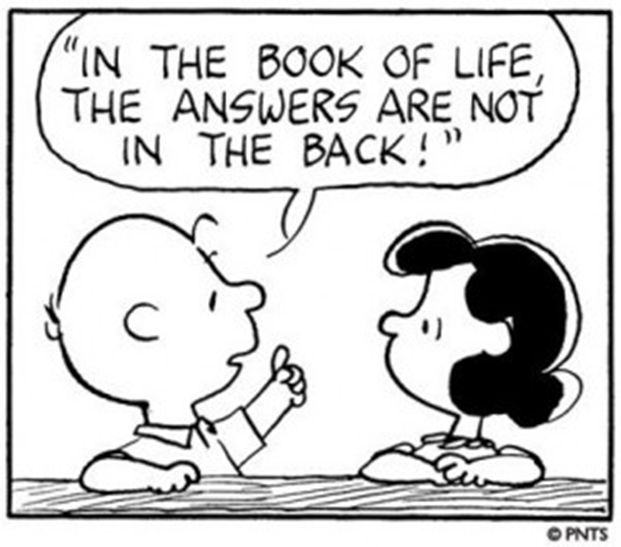
\includegraphics[width=1\linewidth]{ap-pic.png}
	\end{center}
\end{marginfigure}

\section{Fairmont State School of Education Conceptual Framework}
The mission of the Fairmont State University School of Education (FSU SoE) is to prepare reflective and responsive educators who possess the knowledge, skills, and dispositions to help all students learn. The FSU SoE mission is integrated across the curriculum, field experiences, clinical practice, and assessments of candidates. The conceptual framework (CF) provides the structure and guiding principles that are necessary to accomplish this mission. The five West Virginia Professional Teaching Standards (WVPTS) and their respective functions undergird the knowledge, skills, and dispositions that candidates must possess in order to facilitate learning for all students. Diversity and technology are included in the CF representing themes that are integrated throughout the unit's programs. Demonstrated competencies in the standards/functions empower candidates to function as reflective and responsive educators. The CF is based on research about effective teaching and learning best practices that apply to teacher candidates at the initial level as well as accomplished teachers at the advanced level. The CF and the WVPTS also are central guiding elements of the FSU Professional Development School (PDS) Partnership that provides a critical structure and context for teacher education and educator professional development.

\begin{center}
\begin{figure}%
  \centerline{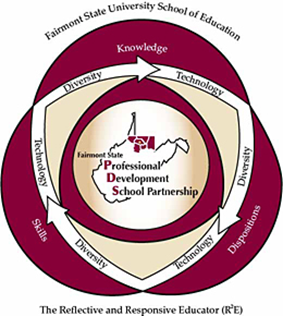
\includegraphics[width=0.5\linewidth]{fsu-cf.png}}
  \caption{Fairmont State University School of Education Conceptual Framework}
  \label{fig:fsu-cf}
\end{figure}
\end{center}

\section{Fairmont State University Policies}

\subsection{Academic Integrity}

Fairmont State values highly the integrity of its student scholars. All students and faculty members are urged to share in the responsibility for removing every situation which might permit or encourage academic dishonesty. Cheating in any form, including plagiarism, must be considered a matter of the gravest concern. Cheating is defined here as: the obtaining of information during an examination; the unauthorized use of books, notes, or other sources of information prior to or during an examination; the removal of faculty examination materials; the alteration of documents or records; or actions identifiable as occurring with the intent to defraud or use under false pretense. Plagiarism is defined here as: the submission of the ideas, words (written or oral), or artistic productions of another, falsely represented as one's original effort or without giving due credit. Students and faculty should examine proper citation forms to avoid inadvertent plagiarism.

\subsection{Disability Services}

Disability services are available to any student, full or part-time, who has a need because of a documented disability. It is the student's responsibility to register for disability services and to provide any necessary documentation to verify a disability or the need for accommodations. Students must provide their professors with a copy of their academic accommodation letter each semester in order to receive accommodations. Faculty, students, and the Office of Disability Services must cooperate to ensure the most effective provision of accommodations for each class.

The Office of Disability Services is located in suite 316 of the Turley Student Services Center 333-3661. For additional information, please visit the Fairmont State University Office of Disability Services webpage at www.fairmontstate.edu/access or call (304) 333-3661.

\end{document}